\documentclass[12pt]{article} 

\usepackage{tikz}
\usepackage{hyperref}

\usetikzlibrary{shapes.geometric, arrows}

\begin{document}

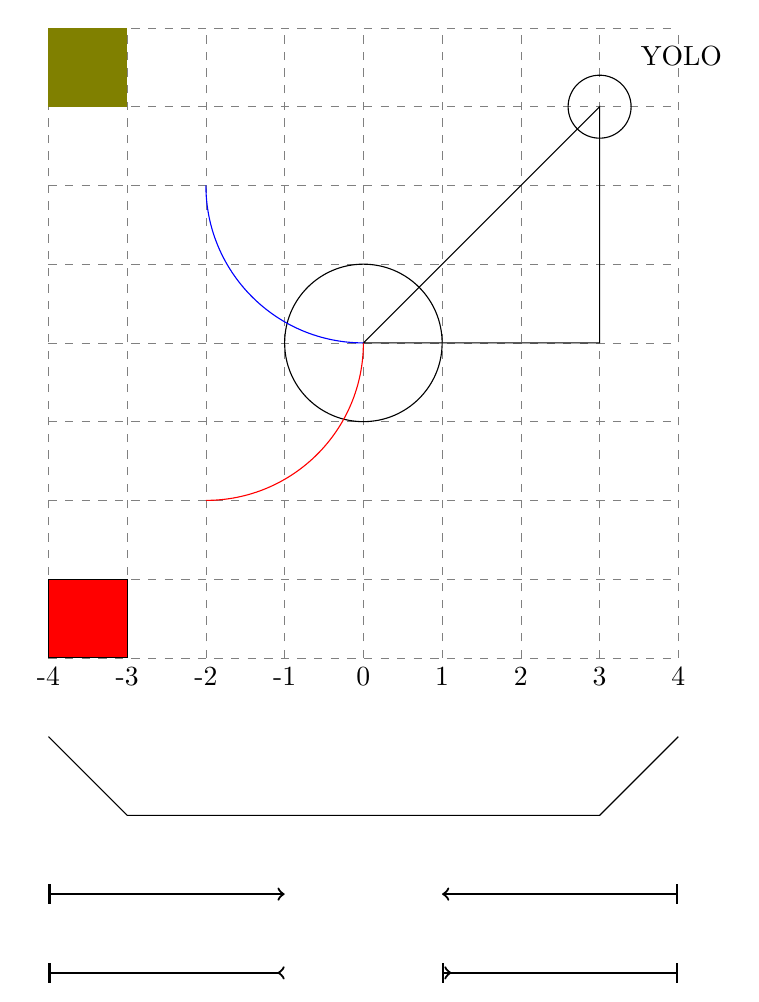
\begin{tikzpicture}
  % Make a grid
  \draw[step=1,gray,very thin, dashed] (-4,-4) grid (4,4);
  % Make a rectangle (`cycle` makes a line between the first and last points)
  \draw (0,0) -- (3,3) -- (3,0) -- cycle;
  % Make a circle at origin with radius 1
  \draw (0,0) circle (1);
  \draw (3,3) circle (0.4);
  % Make an arc with the starting point at origin 
  \draw[red] (0,0) arc (0:-90:2); % from 0 to -90 degrees, with radius=2
  \draw[blue] (0,0) arc (-90:-180:2);
  % Fill a rectangle with 50% red and 50% green
  \fill[red!50!green] (-4,4) rectangle (-3,3);
  % Fill and draw at the same time 
  \filldraw[fill=red, draw=black] (-4,-4) rectangle (-3,-3);
  % Make a line
  \draw (-4,-5) -- (-3,-6) -- (-3,-6) -- (3,-6) -- (4,-5) ;
  % A few arrow styles
  \draw[thick,|->] (-4,-7) -- (-1,-7) ;
  \draw[thick,<-|] (1,-7) -- (4,-7) ;
  \draw[thick,|-<] (-4,-8) -- (-1,-8) ;
  \draw[thick,|>-|] (1,-8) -- (4,-8) ;
  % Add an annotation
  \draw (3.4,3.4) node[anchor=south west] {YOLO} ;
  % Write grid numbers
  \foreach \x in {-4,-3,-2,-1,0,1,2,3,4}
    \draw (\x,-4) node[anchor=north] {\x} ;
\end{tikzpicture}

\section{Overleaf Tutorial Workflow}

This example is taken from: \href{https://www.overleaf.com/learn/latex/LaTeX\_Graphics\_using\_TikZ:\_A\_Tutorial\_for\_Beginners\_(Part\_3)\%E2\%80\%94Creating\_Flowcharts}{here}

\tikzstyle{startstop} = [rectangle, rounded corners, minimum width=3cm, minimum height=1cm,text centered, draw=black, fill=red!30, text width=3cm]
\tikzstyle{io} = [trapezium, trapezium left angle=70, trapezium right angle=110, minimum width=3cm, minimum height=1cm, text centered, draw=black, fill=blue!30, text width=3cm]
% `text width=3cm` forces wrapping of long lines
\tikzstyle{process} = [rectangle, minimum width=3cm, minimum height=1cm, text centered, draw=black, fill=orange!30, text width=3cm]
\tikzstyle{decision} = [diamond, minimum width=3cm, minimum height=1cm, text centered, draw=black, fill=green!30]
\tikzstyle{arrow} = [thick,->,>=stealth]

\begin{tikzpicture}[node distance=2cm]
\node (start) [startstop] {Start};
\node (in1) [io, below of=start] {Input};
\node (pro1) [process, below of=in1] {Process 1};
\node (dec1) [decision, below of=pro1, yshift=-0.5cm] {Decision 1};
\node (pro2a) [process, below of=dec1, yshift=-1.5cm] {Process 2a text text text text text text text text text text};
\node (pro2b) [process, right of=dec1, xshift=2cm] {Process 2b};
\node (out1) [io, below of=pro2a, yshift=-0.3cm] {Output};
\node (stop) [startstop, below of=out1] {Stop};
\draw [arrow] (start) -- (in1);
\draw [arrow] (in1)   -- (pro1);
\draw [arrow] (pro1)  -- (dec1);
\draw [arrow] (dec1)  -- node[anchor=east] {yes} (pro2a);
\draw [arrow] (dec1)  -- node[anchor=south] {no} (pro2b);
\draw [arrow] (pro2b) |- (pro1);
\draw [arrow] (pro2a) -- (out1);
\draw [arrow] (out1)  -- (stop);
\end{tikzpicture}

\end{document}
